Dans cette partie, nous allons visualiser toutes les cas possibles du jeu, utilisant des diagrammes d'état transition.
\subsection{Description des cas d'utilisation}
Dans cette partie, nous allons visualiser toutes les cas possibles du jeu, utilisant des diagrammes d'état transition.
\subsubsection{Vue d'ensemble}
Ce diagramme permet de situer les différents cas possibles de manière générale. Le détail sera fait dans les parties suivantes.


\begin{figure}[!h]
\centering
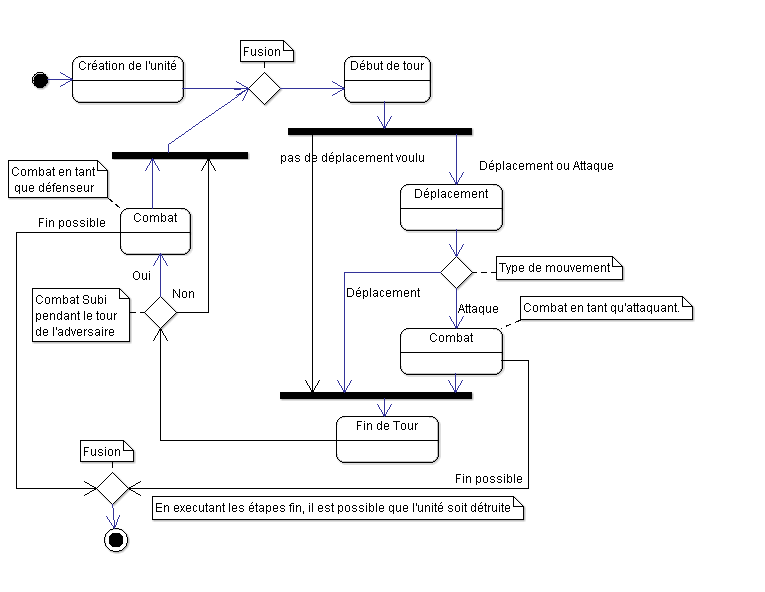
\includegraphics[width=1\textwidth]{img/VueDensemble.png}
\caption{Vue d'ensemble}
\end{figure}

Le cycle de l'unité est le suivant : elle est crée, puis commence son tour, elle peut se déplacer sur une case vide (Déplacement) ou attaquer (Déplacement + Combat). Dans le cas d'un combat, on devra rechercher un défenseur sur la case attaquée. Si aucun n'est trouvé, l'API enverra une erreur. Dans le cas de plusieurs unité présentes sur la case, on choisira l'unité de plus grande défense, et en cas d'égalité, on la choisira au hasard. Cependant, l'unité peut avoir des bonus quelle récupérera en fin de combat (Fin de combat). Après, elle finit son tour, pour en commencer un autre ensuite. Il est possible que l'unité soit attaquée hors de son tour, ainsi, Combat et Fin de combat sont de nouveau appelés pour la défense de l'unité. À chaque combat mené, une unité peut être appelée à perdre des points de vie. Dans le cas de perte de tous les points de vie, l'unité est détruite.

\subsubsection{Déplacement}
Ce diagramme permet de représenter toutes les possibilités de déplacement des différentes unités. On définit la variable d qui représente le coût du déplacement sur la case courante. On définit la constante D qui représente le déplacement autorisé pour chaque pièce en début de tour. Dans l'implémentation proposée, D vaut 2 au premier déplacement de l'unité.

\begin{figure}[!h]
\centering
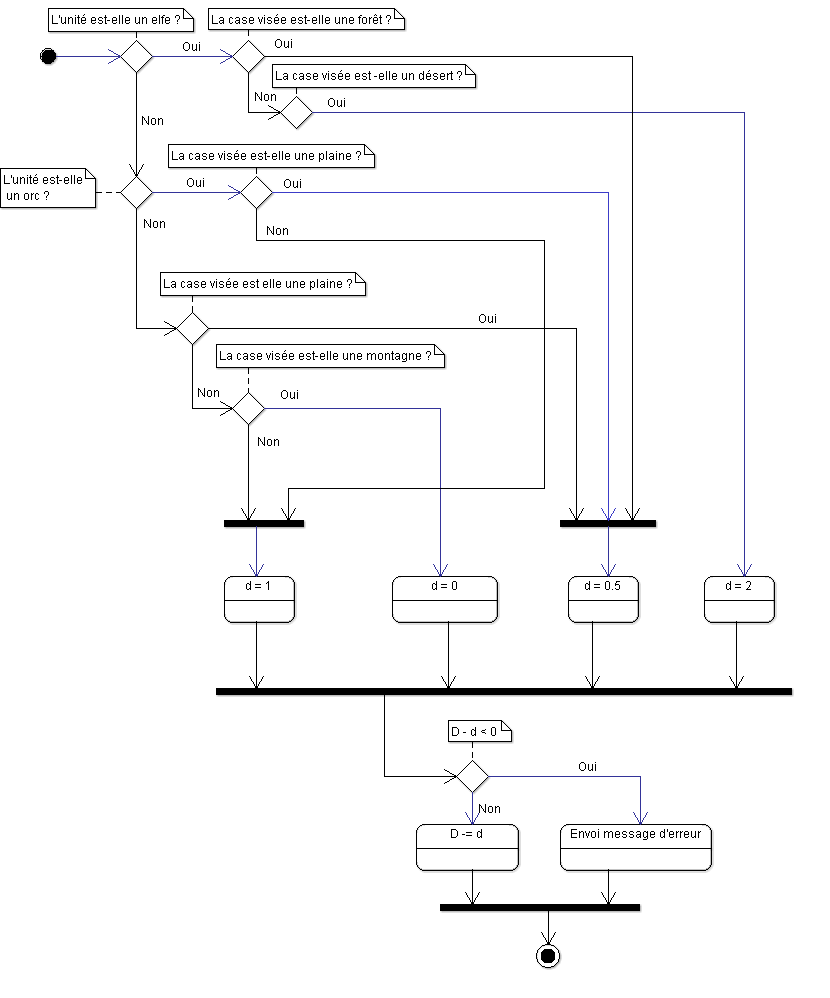
\includegraphics[width=1\textwidth]{img/Deplacement.png}
\caption{Le déplacement d'une pièce}
\end{figure}

On calcule pour commencer la valeur du coût de déplacement sur la case courante d. Pour cela, on teste le type de l'unité, puis le type de case où elle est pour en déduire d. Par exemple, si l'unité est un orc, qui se déplace sur une plaine, le coût de déplacement d n'est que de 0.5. Il est important de noter qu'un nain qui veut se déplacer sur une case montagne aura un coût de déplacement nul.

Après le calcul de d, on vérifie si le déplacement est possible en soustrayant d à D. Le résultat ne doit pas être inférieur à 0. Dans ce cas, le déplacement n'est pas possible et l'API affichera un message d'erreur. Sinon, le déplacement aura lieu, puis on définira D -= d, pour un possible nouveau déplacement.

\subsubsection{Combat}
Ce diagramme permet de représenter toutes les possibilités de combat entre 2 unités. 

\begin{figure}[!h]
\centering
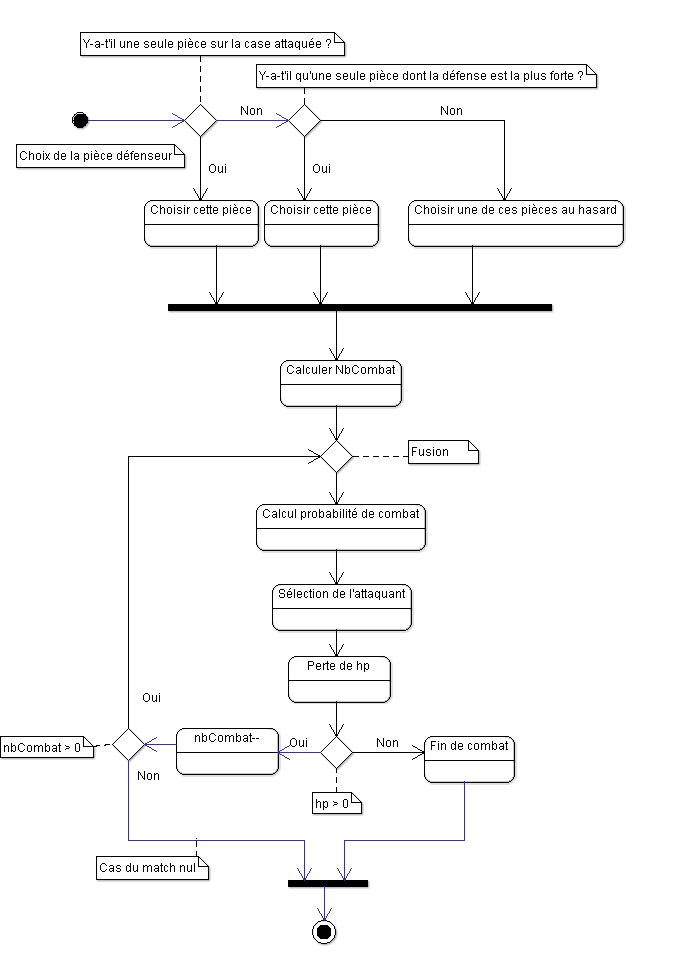
\includegraphics[width=1\textwidth]{img/Combat.png}
\caption{Les combats d'une pièce}
\end{figure}

Premièrement, on calcule le nombre de tours de combats nécessaires maximum nbCombat = Max(3,X+2), X étant le nombre de points de vie maximum des unités au combat. Ensuite, on calcule les probabilités de combat. On tire ensuite un nombre au hasard entre 1 et 100. Si le nombre appartient à la tranche du joueur ciblé (35 % = [0,35[), il peut infliger des blessures à son adversaire, et inversement. Ainsi, le perdant du tour de combat perd Y vies, Y étant la valeur d'attaque de l'unité pondéré par le pourcentage de vie de l'unité. Si l'unité compte 2 points de vie, sachant qu'elle a démarré avec 5 points de vie, alors l'attaque sera multipliée par 40%. Le compteur de nombre de combats est décrémenté et on regarde ensuite s'il reste encore des tours de combat. Si oui, on refait le calcul de probabilité, et ainsi de suite. Sinon, on stoppe le combat par un match nul. L'attaquant ne bouge pas. Son tour est terminé. Si durant le combat, une unité n'a plus de point de vie, elle est détruite.

subsubsection{Calcul de probabilités de combat}
La première chose réalisée est le calcul de 2 rapports de force entre les pièces. Ils concernent respectivement l'attaque de la première pièce et la défense de la deuxième pièce, et inversement. Par exemple, si l'attaque et la défense analysée sont égales, alors le rapport de force vaudra 50%. Ensuite, on soustrait les deux rapports de force distinctement à 100. On multiplie ensuite les rapports de force, et on ajoute le résultat au rapport de force de l'attaquant, et on le soustrait le résultat au rapport de force du défenseur. On obtient donc la probabilité finale.
Par exemple, Si l’attaquant a 4 en attaque et l’attaqué a 4 en défense
(en tenant compte des bonus de terrain et du nombre de points de vie restant), l’attaquant à 50%
de malchance de prendre des dégats. S’il a 3 att. contre 4 déf., le rapport de force est de 75% : 3/4
= 25%, 25% de 50% = 12.5%, 50%+12.5% = 62.5% chances pour l'attaquant et 50-12.5 = 37.5% chances pour le défenseur.

subsubsection{Fin de combat}

Ce diagramme représente les possibilités de jeu en fin de combat. 

\begin{figure}[!h]
\centering
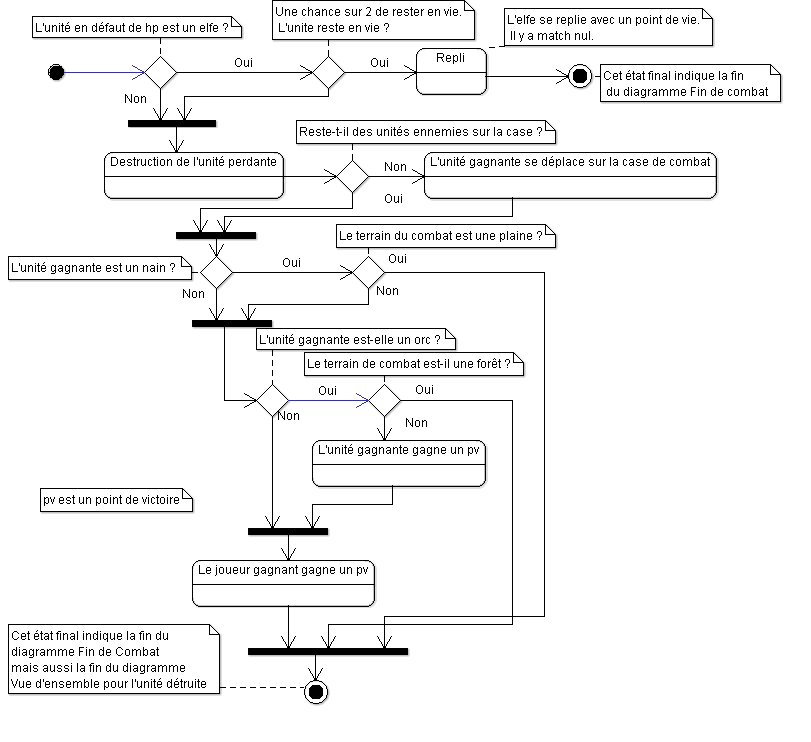
\includegraphics[width=1\textwidth]{img/FinDeCombat.png}
\caption{Les cas de fin de combat d'une pièce}
\end{figure}

En cas de destruction d'unité à la suite d'un combat, qu'il soit défensif ou attaquant, l'unité peut avoir droit à des bonus/malus, selon son type et la case sur laquelle il a gagné le combat. Par exemple, une unité nain ne peut faire gagner de points de victoire. Dans tous les autres cas, toutes les unités gagnent un point de victoire. Il leur est ensuite possible de gagner un autre point de victoire, si l'unité est un est un orc placé sur une case Forest, un point de victoire lui est attaché. Ces points sont cumulables et seront ajoutés au total de points de victoire en fin de partie. Attention, si l'unité orc meurt, le point de victoire bonus disparaît avec lui. 

subsection{Interactions entre les différentes composantes du jeu}
Dans cette partie, nous allons présenter par des diagrammes d"interaction comment fonctionne plus profondément le jeu. Nous commencerons par la procédure d'initialisation du jeu.

subsubsection{Initialisation}

\begin{figure}[!h]
\centering
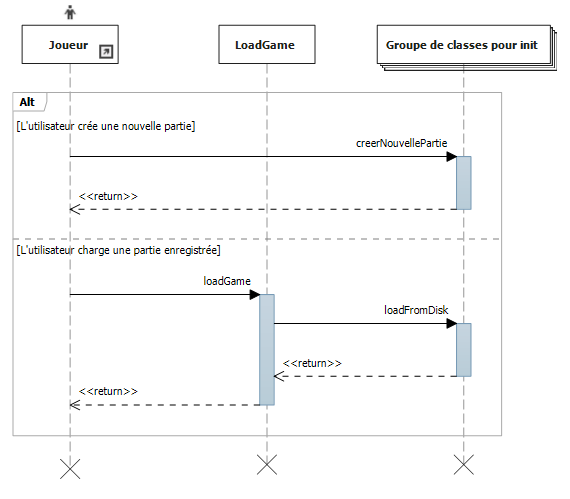
\includegraphics[width=1\textwidth]{img/LoadInitDiagram.png}
\caption{Chargement du jeu par diagramme de séquence}
\end{figure}

\begin{figure}[!h]
\centering
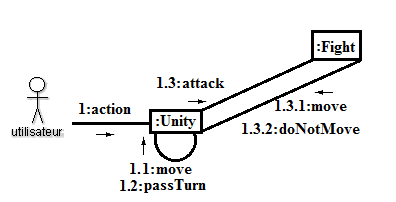
\includegraphics[width=1\textwidth]{img/comm2.png}
\caption{Les combats d'une pièce par diagramme de communication}
\end{figure}

Ce diagramme de séquence permet de différencier la charge d'une partie de la création d'une partie. On voit qu'on ne peut pas charger et créer en même temps. Le Groupe de classes pour init est décrit dans les prochains diagrammes.

\begin{figure}[!h]
\centering
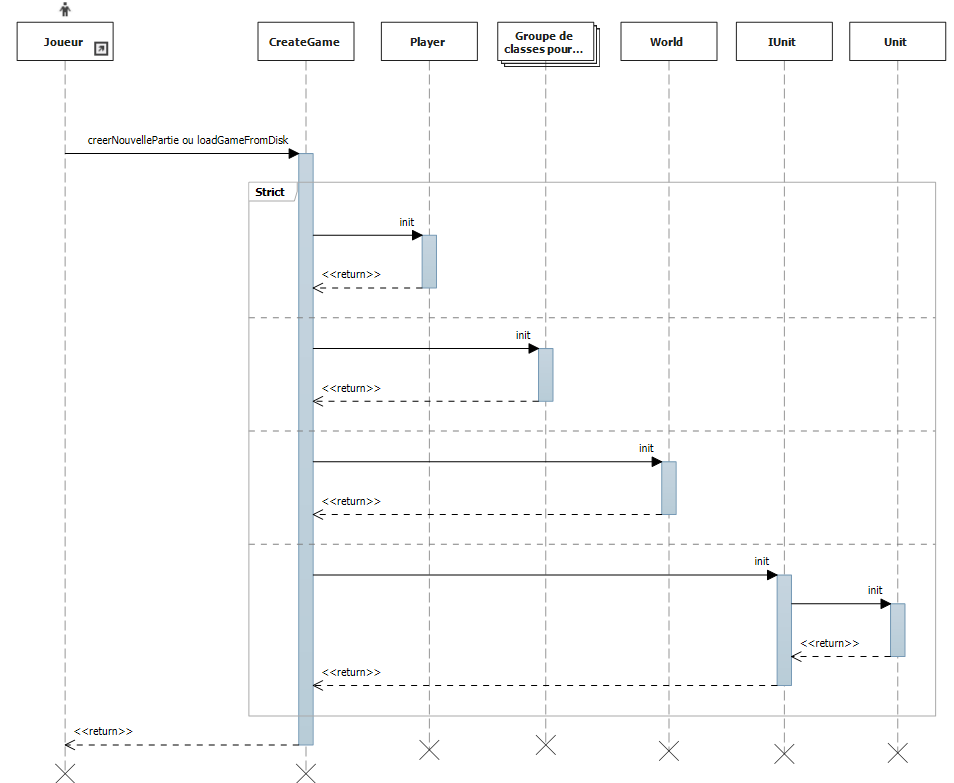
\includegraphics[width=1\textwidth]{img/InitAll.png}
\caption{Initialisation du jeu}
\end{figure}

Dans ce diagramme de séquence, on peut voir l'ordre de création des objets. CreateGame initialise Player, puis le Board, puis World, puis IUnit, qui prend en charge Unit.

Img InitBoard
Dans ce diagramme de séquence, on peut voir l'ordre de création du Board, avec l'appel à une interface, qui apprelera un monteur qui créera les cases pour l'AbstractBoard, qui initialisera les cases Tiles et leur Position associée.

subsubsection{Combats et déplacements}
Ce diagramme de séquence présente les actions possibles. 

\begin{figure}[!h]
\centering
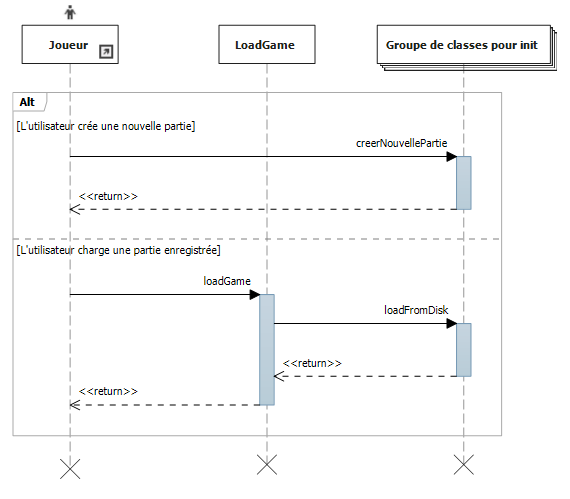
\includegraphics[width=1\textwidth]{img/LoadInitDiagram.png}
\caption{Initialisation du jeu par diagramme de séquence}
\end{figure}

\begin{figure}[!h]
\centering
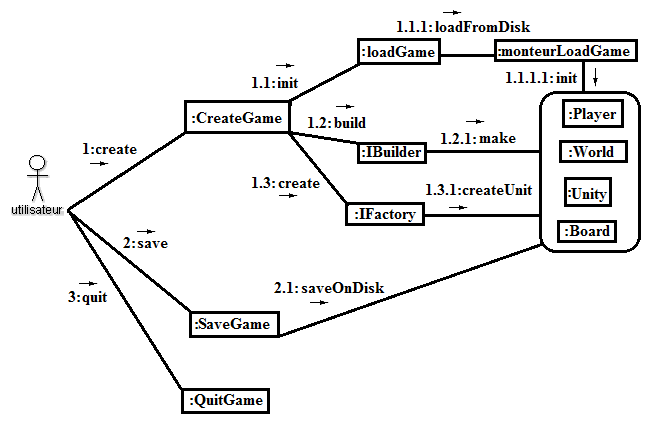
\includegraphics[width=1\textwidth]{img/com.png}
\caption{Initialisation du jeu par diagramme de communication}
\end{figure}

Une unité peut soit gagner le combat, ou le perdre ou faire match nul. Dans le cas de la défaite, on tue l'unité si ses hp sont plus petits que 0.Sinon, comme dans le cas du match nul, on ne fait rien. Dans le cas de la victoire, on bouge sur la case de combat si elle est libre, et on fait les traitements de victoire. Une unité peut aussi bouger. Un joueur perd la partie s'il n'a plus aucune unité.